\documentclass{standalone}
%-----------------------------------------------------------------------------%
%%% Color %%%
\usepackage{xcolor}
\definecolor{myred}{RGB}{229,0,0}
\definecolor{myblue}{RGB}{0,98,144}
\definecolor{myyellow}{RGB}{246,182,50}
\newcommand{\red}[1]{\textcolor{myred}{#1}}
\newcommand{\blue}[1]{\textcolor{myblue}{#1}}
\newcommand{\yellow}[1]{\textcolor{myyellow}{#1}}
%-----------------------------------------------------------------------------%
%%% TikZ %%%
\usepackage{tikz}
\usetikzlibrary{perspective}
\usetikzlibrary{calc}
% \usetikzlibrary{positioning}
% \usetikzlibrary{patterns}
% \usetikzlibrary{fit}
% \usetikzlibrary{angles,quotes}
% \usetikzlibrary{intersections}
% \usetikzlibrary{decorations.markings}
%-----------------------------------------------------------------------------%
%%% TikZ: Mark Angles %%%
\newcommand{\MarkRightAngle}[5][]{
\draw[#1] let \p1=($(#4)-(#3)$), \p2=($(#5)-(#4)$), \p0=($0*(\p1)$) in
(#4)--($(#4)!#2!(#3)$)--++($(\p0)!#2!(\p2)$)--++($(\p0)!#2!(\p1)$)--cycle;}
%-----------------------------------------------------------------------------%

\begin{document}

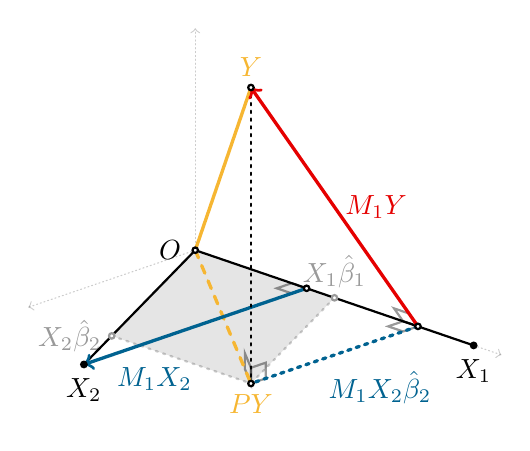
\begin{tikzpicture}[thick,line cap=round,3d view={135}{20}]
	\tikzstyle{bai}=[solid,circle,draw,inner sep=.07em,fill=white];
	\tikzstyle{hei}=[solid,circle,draw,inner sep=.07em,fill];
	\coordinate (O)     at (0,0,0);
	\coordinate (x)     at (3,0,0);
	\coordinate (y)     at (0,5.5,0);
	\coordinate (z)     at (0,0,3);
	\coordinate (X1)    at (0,5,0);
	\coordinate (X2)    at (4,2,0);
	\coordinate (Y)     at (3,4,4);
	\coordinate (Yhat)  at (3,4,0);
	\coordinate (M1Y)   at (0,4,0);
	\coordinate (M1X2)  at (0,2,0);
	\coordinate (beta1) at (0,2.5,0);
	\coordinate (beta2) at (3,1.5,0);
	%%
	\path[fill=black,opacity=0.1] (O) -- (beta1) -- (Yhat) -- (beta2) --cycle;
	\draw[opacity=0.2,dotted] (beta1) node[above,opacity=0.4]{$X_1\hat\beta_1$} -- (Yhat);
	\draw[opacity=0.2,dotted] (beta2) node[left,opacity=0.4]{$X_2\hat\beta_2$} -- (Yhat);
	%%
	\begin{scope}[opacity=0.4]
		\MarkRightAngle[black]{0.2cm}{O}{M1Y}{Y}
		\MarkRightAngle[black]{0.2cm}{O}{M1X2}{X2}
		\MarkRightAngle[black]{0.2cm}{O}{M1Y}{Yhat}
		\MarkRightAngle[black]{0.2cm}{O}{Yhat}{Y}
		\MarkRightAngle[black]{0.2cm}{M1Y}{Yhat}{Y}
		% \MarkRightAngle[black]{0.2}{beta1}{Yhat}{Y}
		% \MarkRightAngle[black]{0.2}{beta2}{Yhat}{Y}
	\end{scope}
	%%
	\begin{scope}[opacity=0.2,densely dotted,thin,->]
		\draw (O) -- (x);
		\draw (O) -- (y);
		\draw (O) -- (z);
	\end{scope}
	%%
	\draw (O) -- (X1);
	\draw (O) -- (X2);
	\draw[very thick,myyellow] (O) -- node[pos=1,above]{$Y$} (Y);
	\draw[very thick,myyellow,dashed] (O) -- node[pos=1,below]{$PY$} (Yhat);
	\draw[very thick,myblue,dotted] (M1Y) -- node[pos=0.6,below right]{$M_1X_2\hat\beta_2$} (Yhat);
	\draw[very thick,myblue,->] (M1X2) -- node[pos=0.9,below right]{$M_1X_2$} (X2);
	\draw[dotted] (Y) -- (Yhat);
	\draw[very thick,myred,->] (M1Y) -- node[pos=0.5,right]{$M_1Y$} (Y);
	%% Nodes
	\node[bai,label=left:{$O$}] at (O) {};
	\node[draw=black!40,bai] at (beta1) {};
	\node[draw=black!40,bai] at (beta2) {};
	\node[bai] at (M1Y) {};
	\node[hei,label=below:{$X_1$}] at (X1) {};
	\node[hei,label=below:{$X_2$}] at (X2) {};
	\node[bai] at (Yhat) {};
	\node[bai] at (M1X2) {};
	\node[bai] at (Y) {};
\end{tikzpicture}

\end{document}
